\scanpage{108}
\mspage{107}\margin{\figure{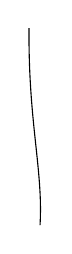
\begin{tikzpicture}\draw(0,0)..controls(.04,.7)and(-.15,1.3)..(-.14,2.5);\end{tikzpicture}}}
\deleted{
\uline{Corollaire} \unsure{4|2}.9.10. Soit $f:X\longrightarrow Y$ un morphisme \deleted{de}
\inserted{de type fini,} \deleted{\unsure{propre}} où $Y$ loc. noeth., $y\in Y$, on suppose
$f$ \unsure{univ.} ouvert en les \unsure{pts} de $X_y$, et $X_y$ séparable.
\deleted{Alors, la fonction $\unsure{y}\mapsto\unsure{\pi_0(y)}$}
\inserted{Pour tt $z\in\unsure{Z|Y}$, soit $\pi(z)=\unsure{\mathrm{nb}^{\mathrm{re}}}$ de}
\unsure{composantes} connexes \unsure{géom} de $X_z$. Alors la fonction
$z\mapsto\unsure{\pi(z)}$ est
\deleted{\unsure{continue} \unsure{en} \unsure{y}}
\inserted{\unsure{$\frac12$} \unsure{continue}}
\unsure{en} \deleted{\unsure{un} \unsure{voisinage}} de $y$.
[elle est continue en $y$].

\deleted{La \deleted{\unsure{fonction}} \unsure{définie} \unsure{ci-dessus} est ``$\frac12$ continue
\unsure{semi-inférieurement}'', par la ``\unsure{th.} de connexité''.}

\deleted{\unsure{Il reste} \illegible{4} \unsure{qu'elles sont}
\unsure{les composantes} \unsure{supérieures} \unsure{à} \unsure{ceux}
\unsure{connexes} (\unsure{comme} elles sont \unsure{constr.}).}

Pour \unsure{tout} \unsure{pt} géom $y'$ de $y$,
on a $\pi(y)\geq\pi(y')$. La \unsure{propriété}
\unsure{précitée} nous ramène alors
au cas où $Y$ est le spectre d'un
anneau de valuation discrète, et où
les \unsure{composantes} connexes de $\unsure{X_0},\unsure{X_1|X_\eta}$
\unsure{sont} géométriques. On peut \unsure{ainsi}
\unsure{supposer} $X$ connexe, \unsure{alors}
$\unsure{X_1|X_\eta}$ est connexe,
\deleted{$\unsure{X_0}$ \unsure{a} \unsure{fini}}
donc \deleted{$\pi(\unsure{X_0})$} $\pi(X_1)=1$,
\deleted{\unsure{donc}} \uline{et}
\uline{comme} $X_0\neq\varnothing$, on a fini.
}
\margin{\figure{\begin{tikzpicture}
\draw (0,0)--(0,1.5);\fill (0,0) circle (.04);
\end{tikzpicture}}}
\margin{\figure{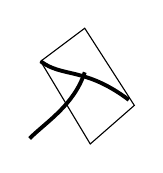
\begin{tikzpicture}[scale=.7]
\draw (0,1.5)--(.8,2.1)--(1.7,.7)--(.9,0)--cycle;
\draw[line width=1.4pt] (0,1.5)..controls(.4,1.2)and(.8,1.4)..(1.6,.8);
\draw[line width=1.4pt] (.8,1.3)..controls(.6,.7)and(.1,.4)..(-.2,.1);
\end{tikzpicture}}}
\margin{\figure{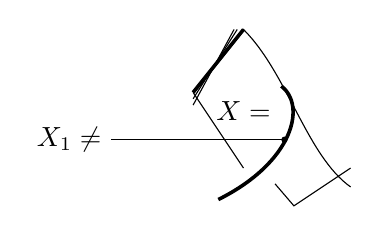
\begin{tikzpicture}[scale=.8]
\draw (0,1.7)--(.8,2.7)..controls(1.5,2)and(1.8,.7)..(2.5,.2);
\draw (0,1.7)--(.8,.5);\draw (1.3,.25)--(1.6,-.1)--(2.5,.5);
\draw[line width=1.3pt] (0,1.7)--(.8,2.7);
\draw (0,1.6)--(.7,2.7);\draw (0,1.5)--(.65,2.7);
\draw[line width=1.3pt] (.4,0)..controls(1.6,.6)and(1.8,1.5)..(1.4,1.8);
\draw (-1.3,.95)--(1.45,.95);\fill (1.45,.95) circle (.05);
\node[left] at(-1.3,.95){$X_1\neq\varnothing$};
\node at(.8,1.4){$\unsure{X=\varnothing}$};
\end{tikzpicture}}}
\margin{\figure{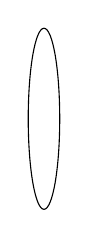
\begin{tikzpicture}\draw (0,0) ellipse (.2 and 1.15);\end{tikzpicture}}}
\deleted{\diagram{\begin{tikzcd}[column sep=small,row sep=large]
0\arrow[r]\arrow[dr,dash,bend right=30]&
N\arrow[r]\arrow[d,dash,bend right=20]&
M\arrow[r,dash]\arrow[d,dash,bend right=15]&
M/N\arrow[r,dash]\arrow[d,dash,bend left=25]&0\arrow[dl,dash,bend left=35]\\
0\arrow[r,dash]&N'+N\arrow[r,dash]&M'+M\arrow[r]&P'+P\arrow[r,dash]&0
\end{tikzcd}}}
\margin{\unsure{Lem} \unsure{d'homologie}}
\margin{\figure{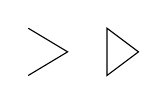
\begin{tikzpicture}\draw (0,0)--(.5,.3)--(0,.6);\draw (1,0)--(1.4,.3)--(1,.6)--cycle;\end{tikzpicture}}}

